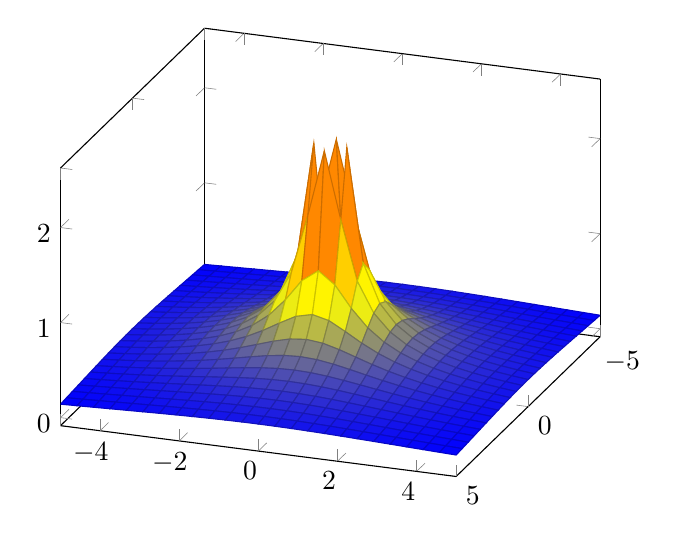
\begin{tikzpicture}
\begin{axis}[
 view={110}{30},
    unbounded coords=jump,
    z filter/.expression={
        z>20 ? nan : z
    }
]
\addplot3[surf,]{sqrt((-x/(x^2+y^2))^2+(y/(x^2+y^2))^2)};
\end{axis}
\end{tikzpicture}
\caption*{Campo escalar del modulo}